\section{Your first Laplace Transform calculations}

\subsection*{Resources}
\begin{itemize}
    \item Videos: The \textbf{four} Khan-academy videos starting at \url{https://www.khanacademy.org/math/differential-equations/laplace-transform/laplace-transform-tutorial/v/laplace-transform-1} % 8m+7:30+10+9 = 35:30
\end{itemize}

\subsection*{Comment}
The Laplace Transform is a powerful technique that has many uses beyond solving ODE's. It can however appear a bit abstract at first. Becoming comfortable with controlling and manipulating the transform will help provide confidence when using it to solve ODE's. The four videos in the resources above provide an excellent starting point for getting you comfortable with this powerful technique.

\subsection*{Challenge}
1. Calculate $\lap{1}$

2. Calculate $\lap{at}$

3. Calculate $\lap{Cos(at)}$

\subsection*{Solution}
To check your answer, substitute $s=1$ and $a=2$ into your final solution.

1. 1

2. 2

3. $\frac{1}{5}$




%%%%%%%%%%%%%%%%%%%%%%%%%%%%%%%%
\newpage
%%%%%%%%%%%%%%%%%%%%%%%%%%%%%%%%
\section{Laplace transform of a 3rd derivative}

\subsection*{Resources}
\begin{itemize} % Total video time: 20m
    \item Video I: \url{https://www.khanacademy.org/math/differential-equations/laplace-transform/properties-of-laplace-transform/v/laplace-transform-5} % 11:30
    \item Video II: \url{https://www.khanacademy.org/math/differential-equations/laplace-transform/properties-of-laplace-transform/v/laplace-transform-6} % 9:30
\end{itemize}

\subsection*{Challenge}
1. Calculate $\displaystyle \frac{d^3}{dt^3} \left( t e^{a t} \right)$

2. Given
\begin{equation}
    \lap{t e^{a t}} = \frac{1}{(a-s)^2}
\end{equation}
determine $\lap{3a^2 e^{at} + a^3te^{at}}$

\subsection*{Solution}
To check your answer, substitute $s=1$ and $a=2$ into your final solution.

-4




%%%%%%%%%%%%%%%%%%%%%%%%%%%%%%%%
\newpage
%%%%%%%%%%%%%%%%%%%%%%%%%%%%%%%%
\section{Shifting a transform}

\subsection*{Resources}
\begin{itemize}
    \item Video \url{https://www.khanacademy.org/math/differential-equations/laplace-transform/properties-of-laplace-transform/v/more-laplace-transform-tools} %11m
\end{itemize}

\subsection*{Challenge}
Given
\begin{equation}
    \lap{Cosh(at)} = \frac{s}{s^2-a^2}
\end{equation}

1. What is $\lap{e^{3t} Cosh(5t)}$?

2. What is $f(t)$ in the equation $\lap{f(t)} = \frac{s-4}{(s-4)^2-100}$?

\subsection*{Solution}
To check your answer, substitute $s=2$ and $t=2$ as appropriate:

1. $0.0417$

2. $7.23 \times 10^{11}$




%%%%%%%%%%%%%%%%%%%%%%%%%%%%%%%%
\newpage
%%%%%%%%%%%%%%%%%%%%%%%%%%%%%%%%
\section{L'H\^opital's rule}

\subsection*{Resources}
\begin{itemize}
    \item \url{https://en.wikipedia.org/wiki/L\%27H\%C3\%B4pital\%27s_rule}
\end{itemize}

\subsection*{Challenge}
1. Use L'H\^opital's rule to determine the limit of
\begin{equation}
    t e^{-st}
\end{equation}
as $x \rightarrow 0$.

2. Considering the case of
\begin{equation}
    \frac{t^n}{e^{st}}
\end{equation}
if we differentiate $n$ times with respect to $t$, what is the power of $t$ in the numerator? Note that $e^{st}$ is always constant, so by repeated differentiation we can apply L'H\^opital's rule even for $t^n$.

\subsection*{Solution}
1. \hash{ww}{76c8d4}

2. \hash{xx}{1592d7}




%%%%%%%%%%%%%%%%%%%%%%%%%%%%%%%%
\newpage
%%%%%%%%%%%%%%%%%%%%%%%%%%%%%%%%
\section{Laplace Transformation of the unit step function}

\subsection*{Resources}
\begin{itemize}
    \item \url{https://www.khanacademy.org/math/differential-equations/laplace-transform/properties-of-laplace-transform/v/laplace-transform-of-the-unit-step-function} % 24m
\end{itemize}

\subsection*{Challenge}
Considering $U_c$ as the unit step-function at $c$, calculate the following Laplace transformations:

1. $\displaystyle \lap{U_0}$

2. $\displaystyle \lap{U_c}$

3. A 1-second pulse function starting at time $t=1$ with value $f(y)=1$ as shown in the graph below:
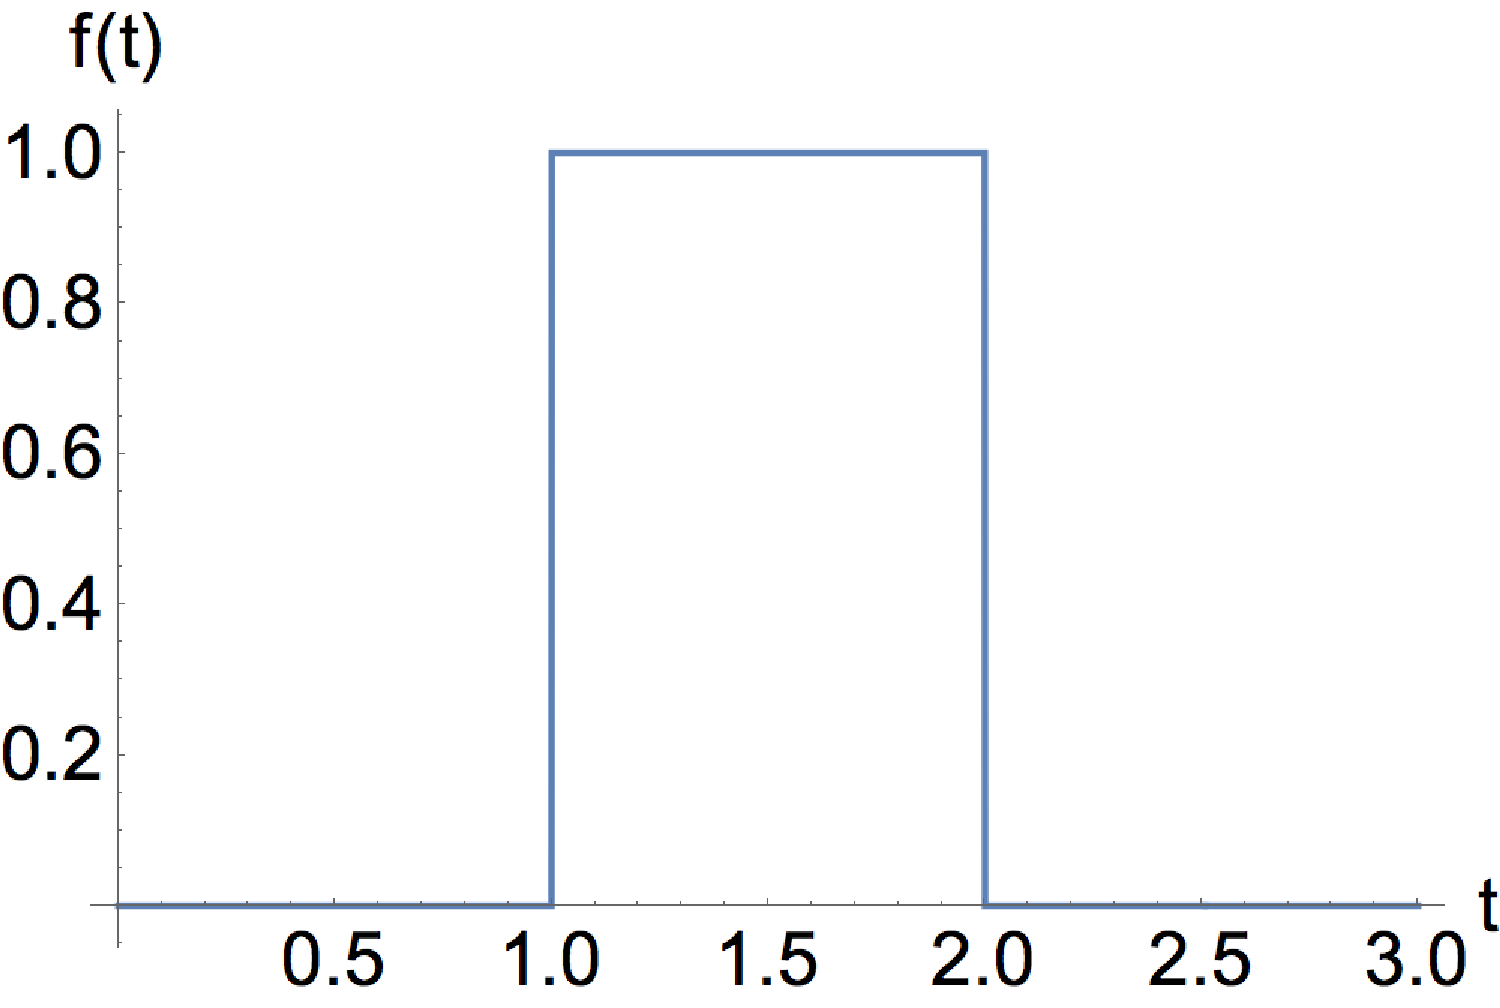
\includegraphics[scale=0.5]{pulse.png}

4. $\displaystyle \lap{U_\pi(t) cos(t-\pi)}$

\subsection*{Solution}
To check your answers, substitute $c=1$ and $s=2$ as appropriate.

1. \hash{yy}{39574c}

2. 0.0677

3. 0.0585

4. $7.470 \times 10^{-4}$




%%%%%%%%%%%%%%%%%%%%%%%%%%%%%%%%
\newpage
%%%%%%%%%%%%%%%%%%%%%%%%%%%%%%%%
\section{Inverse Laplace Transform}

\subsection*{Resources}
\begin{itemize}
    \item \url{https://www.khanacademy.org/math/differential-equations/laplace-transform/properties-of-laplace-transform/v/inverse-laplace-examples} % 19m
\end{itemize}

\subsection*{Comment}
Being able to reversing the Laplace transform is a crutial skill required for applying it to solving ODE's. It can be a little confusing at first however, so I recommend to take your time to understand the essential steps involved thoroughly, as this will then give you greater confidence when you come to apply this to solving ODE's. To this end, the video listed in the resource is a fantastic introduction to this.

\subsection*{Challenge}
Determine the function $f(t)$ by finding the inverse of the following Laplace transforms:

1. $\displaystyle F(s)=\frac{1}{(s-1)^2}$

2. $\displaystyle F(s)=\frac{1-s}{s^2}$

3. $\displaystyle F(s)=\frac{2 e^{-2s}}{s^2-2s+2}$

4. $\displaystyle F(s)=\frac{6}{2+s^4}$

5. $\displaystyle F(s)=\frac{120+6s^3}{s^6}$

6. $\displaystyle F(s)=\frac{e^{12-3s}}{s-4}$


\subsection*{Solution}
To check your answers, subsititute $t=2$ into your final answer. If there is a unit-step in your solution, preceed your numerical answer with ``u(c)'' where ``c'' is the position of the unit step. So for example, an answer of $U_5 t^2$ would be entered as ``u(5.00)4.00'' (all numbers to two decimal places). An answer without a unit-step would just be entered to two decimal places (eg, ``4.00'' in the previous example).

1. Hash = 5cacdb\ldots

2. Hash = 41cf26\ldots

3. Hash = 45c11e\ldots

4. Hash = 9ffc7a\ldots

5. Hash = 766fd0\ldots

6. Hash = 6a7dc6\ldots
